\documentclass[french]{beamer}

\usepackage[utf8]{inputenc}
\usepackage[T1]{fontenc}
\usepackage{lmodern}
\usepackage{babel}
\usepackage{tikz}
\usepackage{graphicx}
\usetikzlibrary{arrows}

\usetheme{PaloAlto}

\tikzset{
  treenode/.style = {align=center, inner sep=0pt, text centered,
    font=\sffamily},
  arn_equi/.style = {treenode, circle, white, draw=green, fill=green, text width=1em},
  arn_notequi/.style = {treenode, circle, white, draw=red,fill=red, text width=1em},
  arn_new/.style = {treenode, circle, white, draw=blue,fill=blue, text width=1em},
  arn_null/.style = {treenode, rectangle, draw=black,minimum width=0.5em, minimum height=0.5em}
}



%Pour le TITLEPAGE
\title{Compression}
\subtitle{Projet Mathématiques et Informatique}
\author[]{LABADENS Lucas, \\ MARINO Isabelle}
\date{13 Juin 2016}
\institute[L3 S6-- Informatique]{Université Paris 7 Diderot}


\begin{document}

\begin{frame}
	\titlepage
\end{frame}

\begin{frame}
	\frametitle{Sommaire}
	\tableofcontents	
\end{frame}

\section{La compression: définition }
\begin{frame}{La Compression}
	\textbf{Plusieurs types de compression} :
	\begin{itemize}
	\item<2-3>  Compression sans perte de données
	\item<3>  Compression avec perte de données
	\end{itemize}
\end{frame}

\section{Huffman}
\begin{frame}{Huffman}
	\begin{center}
	\textbf{Caractéristique} :\\
	
	\begin{itemize}
	\item  Un codage entropique
	\item  repose sur la redondance de caractère
	\item code un caractère non plus sur un octet mais sur un nombre de bit 
	\end{itemize}
	\end{center}
\end{frame}

\begin{frame}{Compression}

	\textbf{Etape} :\\
	
\begin{itemize}
	\item compte des redondances de caractères
	\item création de l'arbre de compression en fonction des poids des caractères :
		\begin{itemize}
			\item on crée des feuilles qui sont des poids munie d'un caractère
			\item on relie les deux feuilles de poids de plus faible par un nœud qui est un poids muni d'un fils gauche et droit
			\item on relie les poids les deux poids les plus faibles par un nouveau  jusqu'à ne plus avoir qu'un seul nœud
		\end{itemize}
	\item récupération des nouveaux codes de chaque caractère
	\item relecture du fichier pour écrire chaque caractère dans le fichier compresser avec son nouveau code
	\item on complète le dernière octet par la convention un 1 puis le nombre de 0 nécessaire
	\end{itemize}

\end{frame}

\begin{frame}{Décompression}
\textbf{Etape} :\\
\begin{itemize}
\item<1-5> récupération de l'arbre de compression
\item<2-5> lecture du fichier compresser bit à bit et parcours de l'arbre :
	\begin{itemize}
		\item<3-5> lecture d'un 0 on se déplace à gauche et sinon à droite
		\item<4-5> lorsque l'on tombe sur une feuille on écrit son caractère associé dans le fichier de décompression
	\end{itemize}
\item<5> attention à ne pas lire les bits complétant le dernière octet du fichier
\end{itemize}
\end{frame}

\begin{frame}{Exemple}
	\begin{center}
	\textbf{Etape 1} \\
	Soit unn texte ou il est écrit :  aaaabcbbce \\
	(a,4) (b,3) (c,2) (e,1)
	\end{center}
\end{frame}
\begin{frame}{Exemple}
	\begin{center}
	\textbf{Etape 2} \\
	\begin{tikzpicture}
	\node (0) at (0,0) {3};
	\node (1) at (-1,-1) {(e,1)};
	\node (2) at (1,-1) {(c,2)};
	\node (3) at (3,-1/2) {(b,3)};
	\node (4) at (5,-1/2) {(a,4)};
	\draw [-,>=latex,](0)--(1) node[pos=0.6,left, above]{0};
	\draw [-,>=latex,](0)--(2) node[pos=0.6,right, above]{1};
	\end{tikzpicture}	
	\end{center}
\end{frame}
\begin{frame}{Exemple}
	\begin{center}
	\textbf{Etape 2} \\
	\begin{tikzpicture}
	\node (0) at (0,0) {3};
	\node (1) at (-1,-1) {(e,1)};
	\node (2) at (1,-1) {(c,2)};
	\node (3) at (2,0) {(b,3)};
	\node (4) at (5,-1/2) {(a,4)};
	\node(5) at 	(1,1){6};
	\draw [-,>=latex,](0)--(1) node[pos=0.6,left, above]{0};
	\draw [-,>=latex,](0)--(2) node[pos=0.6,right, above]{1};
	\draw [-,>=latex,](5)--(0) node[pos=0.6,left, above]{0};
	\draw [-,>=latex,](5)--(3) node[pos=0.6,right, above]{1};
	\end{tikzpicture}	
	\end{center}
\end{frame}
\begin{frame}{Exemple}
	\begin{center}
	\textbf{Etape 3} \\
	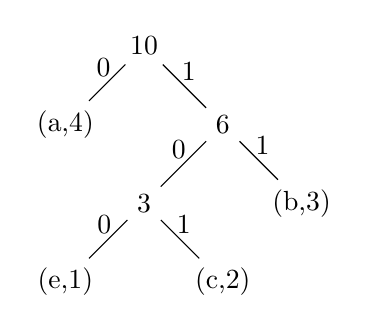
\begin{tikzpicture}
	\node (0) at (0,0) {3};
	\node (1) at (-1,-1) {(e,1)};
	\node (2) at (1,-1) {(c,2)};
	\node (3) at (2,0) {(b,3)};
	\node (4) at (-1,1) {(a,4)};
	\node(5) at 	(1,1){6};
	\node(6) at (0,2){10};
	\draw [-,>=latex,](0)--(1) node[pos=0.6,left, above]{0};
	\draw [-,>=latex,](0)--(2) node[pos=0.6,right, above]{1};
	\draw [-,>=latex,](5)--(0) node[pos=0.6,left, above]{0};
	\draw [-,>=latex,](5)--(3) node[pos=0.6,right, above]{1};
	\draw [-,>=latex,](6)--(4) node[pos=0.6,left, above]{0};
	\draw [-,>=latex,](6)--(5) node[pos=0.6,right, above]{1};
	\end{tikzpicture}	
	\end{center}
\end{frame}
\begin{frame}{Exemple}
\begin{center}

\textbf{Ecriture compresser}\\
les nouveaux codes sont a='0' b='11' c='101' e='100'
\end{center}
\end{frame}
\begin{frame}{Performances}
	\begin{center}
	exemple d'inclusion de graphe 
	%\includegraphics[width=6cm]{structures.png}
	\end{center}
\end{frame}

\section{Lempel-Ziv}
\begin{frame}{Lempel-Ziv}
	\begin{center}
	blabla
	\end{center}
\end{frame}


\begin{frame}{Exemple: Compression}
	\begin{center}
	\end{center}
\end{frame}
\begin{frame}{Exemple: Décompression}
	\begin{center}
	\end{center}
\end{frame}

\begin{frame}{Performances}
	\begin{center}
	\textbf{Plusieurs suites de compression} :
	\begin{itemize}
	\item[]<2>  	blb%\includegraphics[width=6cm]{structures.png}
	\item[]<3>  	nn%\includegraphics[width=6cm]{structures.png}
	\end{itemize}
	\end{center}
\end{frame}



\section{Différences entre les algorithmes}
\begin{frame}{Différences de structures}
	\begin{center}
	%\includegraphics[width=7.9cm]{dependances.png}
	\end{center}
\end{frame}
\begin{frame}{Temps d'exécution à la compression} 
	\begin{center}
	%\includegraphics[width=7.9cm]{dependances.png}
	\end{center}
\end{frame}
\begin{frame}{Temps d'exécution à la décompression}
	\begin{center}
	%\includegraphics[width=7.9cm]{dependances.png}
	\end{center}
\end{frame}

\section{Différences avec les principaux compresseurs}
\begin{frame}{Principales différences}
	\begin{center}
	%\includegraphics[width=10cm]{fonctions.png}
	\end{center}
\end{frame}

\section{Conclusion}
\begin{frame}{Principales différences}
	\begin{center}
	\end{center}
\end{frame}

\end{document}

